% 第3章 经典连续介质力学与近场动力学的联系
\chapter{经典连续介质力学与近场动力学的联系}
\leavevmode\usetikzlibrary{arrows.meta, positioning, calc}

第 2 章在物质点、对力函数与守恒律三个层面建立了近场动力学的完整数学框架，其中线性化本构关系 $f \approx C(\xi)\eta$ 与有效刚度 $k_{\mathrm{eff}}=\int_{H_x}C(\xi)\,dV$ 已经预示了近场量与宏观量之间的对应。然而该框架本质上是非局部的，而工程中广泛使用的经典连续介质力学建立在 Cauchy 应力与局部微分方程之上，两者如何衔接是理论自洽性与数值实现的关键所在。本章的任务即是在第 2 章框架内严格分析这种联系：首先研究近场范围 $\delta\to 0$ 的局部极限，证明近场动力学方程渐近退化为经典弹性方程；其次引入近场动力学应力张量，建立力密度与 Cauchy 应力散度的对应；进而对各向同性键基模型给出 Lam\'e 常数的显式对应，揭示键基泊松比 $1/4$ 的根源；随后讨论渐近相容性的阶与边界层效应；最后建立非局部变分原理与弱形式，为后续耦合方法奠定基础。本章的结果将直接服务于第 4 章对键型 PMB 模型的具体化与参数率定。

\section{局部极限：近场动力学向经典理论的退化}
\label{sec:local-limit}

第 2 章在 2.1 节已经指出，当近场范围 $\delta\to 0$ 时，近场域 $H_x$ 退化为 $x$ 的无穷小邻域，近场动力学方程在形式上趋近于经典局部理论。本节将对这一极限关系进行严格分析。先利用线性化本构与 Taylor 展开将近场力密度在 $\delta\to 0$ 下的渐近行为展开，再证明其首非零项恰好对应 Cauchy 应力散度，最后考察应变能与键伸长率的退化关系，使第 2 章遗留的若干衔接点得到严格证明。

\subsection{线性化本构与位移的 Taylor 展开}
\label{subsec:taylor-expansion}

考虑参考构型 $B$ 中的光滑位移场 $u(x)$，设 $u\in C^2(B)$。对于近场域 $H_x=\{x'\in B:|x'-x|\le\delta\}$ 内的物质点 $x'$，记键的参考相对位置 $\xi=x'-x$，相对位移 $\eta=u(x')-u(x)$。由 Taylor 展开有
\begin{equation}
\label{eq:u-taylor}
\eta_i = u_i(x+\xi)-u_i(x) = \frac{\partial u_i}{\partial x_j}\,\xi_j + \frac{1}{2}\,\frac{\partial^2 u_i}{\partial x_j \partial x_k}\,\xi_j\xi_k + O(|\xi|^3).
\end{equation}
引入小应变张量 $\varepsilon_{ij}=\tfrac{1}{2}(\partial_j u_i+\partial_i u_j)$ 与旋转张量 $\omega_{ij}=\tfrac{1}{2}(\partial_j u_i-\partial_i u_j)$，则位移梯度分解为
\begin{equation}
\label{eq:grad-decomp}
\frac{\partial u_i}{\partial x_j} = \varepsilon_{ij} + \omega_{ij},
\end{equation}
其中 $\varepsilon$ 为对称部分满足 $\varepsilon_{ij}=\varepsilon_{ji}$，$\omega$ 为反对称部分满足 $\omega_{ij}=-\omega_{ji}$。代入式 \eqref{eq:u-taylor} 得
\begin{equation}
\label{eq:eta-decomp-explicit}
\eta_i = (\varepsilon_{ij}+\omega_{ij})\,\xi_j + \frac{1}{2}\,G_{ijk}\,\xi_j\xi_k + O(|\xi|^3),
\end{equation}
其中 $G_{ijk}=\partial_j\partial_k u_i$ 为位移的二阶梯度张量。此式将相对位移分解为应变贡献、旋转贡献与高阶修正三部分，是后续分析局部极限的基础。

在第 2 章式 \eqref{eq:linear-force} 中已经给出线性化对力 $f\approx C(\xi)\,\eta$，其中 $C(\xi)=\partial f/\partial\eta|_{\eta=0}$ 为微模量张量。由反作用条件 \eqref{eq:reaction} $f(-\eta,-\xi)=-f(\eta,\xi)$，对线性化关系两端作变换 $(\eta,\xi)\to(-\eta,-\xi)$ 得 $-C(-\xi)\,\eta=-C(\xi)\,\eta$，从而
\begin{equation}
\label{eq:micro-modulus-even}
C(-\xi) = C(\xi),
\end{equation}
即微模量张量 $C(\xi)$ 是 $\xi$ 的偶函数。这一偶性将在后续证明中反复使用，是积分项奇偶性论证的根源。

\subsection{力密度退化为应力散度}
\label{subsec:force-to-stress-div}

将近场力密度记为
\begin{equation}
\label{eq:force-density-def}
L_i(x) = \int_{H_x} f_i(\eta,\xi)\,dV' = \int_{|\xi|\le\delta} C_{ij}(\xi)\,\eta_j\,dV_\xi,
\end{equation}
其中第二步利用了线性化对力，$dV_\xi$ 表示关于 $\xi$ 的体积分，积分域换元 $x'=x+\xi$ 后变为球 $|\xi|\le\delta$。将式 \eqref{eq:eta-decomp-explicit} 代入得
\begin{equation}
\label{eq:force-density-expand}
L_i = \int_{|\xi|\le\delta} C_{ij}(\xi)\bigl[(\varepsilon_{jk}+\omega_{jk})\,\xi_k + \tfrac{1}{2}\,G_{jkl}\,\xi_k\xi_l + O(|\xi|^3)\bigr]\,dV_\xi.
\end{equation}
对第一项，注意 $C_{ij}(\xi)\,\xi_k$ 在 $\xi$ 固定下关于 $j,k$ 的结构。由于 $C(-\xi)=C(\xi)$ 而 $\xi_k$ 关于 $\xi\to-\xi$ 为奇函数，故 $C_{ij}(\xi)\,\xi_k$ 是 $\xi$ 的奇函数，积分域 $|\xi|\le\delta$ 在变换 $\xi\to-\xi$ 下不变，于是
\begin{equation}
\label{eq:first-term-vanish}
\int_{|\xi|\le\delta} C_{ij}(\xi)\,(\varepsilon_{jk}+\omega_{jk})\,\xi_k\,dV_\xi = (\varepsilon_{jk}+\omega_{jk})\int_{|\xi|\le\delta} C_{ij}(\xi)\,\xi_k\,dV_\xi = 0,
\end{equation}
其中后一个积分为零严格成立，不仅首阶为零。这是因为被积函数 $C_{ij}(\xi)\,\xi_k$ 是 $\xi$ 的奇函数，在对称球域上积分为零。因此力密度的首非零项来自二阶修正
\begin{equation}
\label{eq:second-order-term}
L_i \approx \frac{1}{2}\int_{|\xi|\le\delta} C_{ij}(\xi)\,G_{jkl}\,\xi_k\xi_l\,dV_\xi.
\end{equation}
定义四阶张量
\begin{equation}
\label{eq:modulus-tensor-M}
M_{ijkl} = \frac{1}{2}\int_{|\xi|\le\delta} C_{ij}(\xi)\,\xi_k\xi_l\,dV_\xi,
\end{equation}
则力密度近似为
\begin{equation}
\label{eq:force-density-approx}
L_i \approx M_{ijkl}\,\frac{\partial^2 u_j}{\partial x_k\partial x_l}.
\end{equation}
注意 $M_{ijkl}$ 关于 $k,l$ 对称（因 $\xi_k\xi_l$ 对称），其具体形式取决于 $C(\xi)$ 的各向异性结构。对于各向同性材料，$M_{ijkl}$ 可约化为标准弹性张量的形式，此时力密度恰好等于 $\nabla\cdot\sigma$，其中 $\sigma$ 为 Cauchy 应力张量。这一对应将在 3.2 节引入近场动力学应力张量后严格证明。

值得强调的是，上述退化是 $\delta\to 0$ 的渐近过程，而非简单地将 $\delta=0$ 代入。$\delta=0$ 时近场域为空集，积分恒为零，这一平凡情形无物理意义。正确的理解是：当 $\delta$ 相对于结构的特征尺度 $L$ 充分小时，近场量与非近场量之差为 $O(\delta^2)$ 量级的小量。这一相容性阶数的严格分析见 3.4 节。

\begin{remark}
局部极限的论证关键在于微模量张量 $C(\xi)$ 的偶性 $C(-\xi)=C(\xi)$，而这一偶性直接源于反作用条件。换元 $\xi\to-\xi$ 使对称球域上的奇函数积分为零这一技巧，在第 2 章守恒律的证明中已多次出现，此处再次体现了这一"换元--相消"模式的核心地位。
\end{remark}

\subsection{应变能与伸长率的退化}
\label{subsec:energy-stretch-degrade}

在局部极限下，应变能密度也退化为经典形式。由第 2 章式 \eqref{eq:strain-energy}，近场应变能密度
\begin{equation}
\label{eq:pd-energy-recall}
W = \frac{1}{2}\int_{H_x} w(\eta,\xi)\,dV',
\end{equation}
其中 $w$ 为成对势。对于线性化情形，$w=\tfrac{1}{2}\,\eta\cdot C(\xi)\,\eta$，于是
\begin{equation}
\label{eq:linear-energy}
W = \frac{1}{4}\int_{|\xi|\le\delta} \eta_i\,C_{ij}(\xi)\,\eta_j\,dV_\xi.
\end{equation}
将 $\eta_i\approx\varepsilon_{ik}\xi_k$ 代入（旋转部分 $\omega_{ik}\xi_k$ 的贡献因 $C$ 的偶性与 $\xi$ 的奇性相消而为零），得
\begin{equation}
\label{eq:energy-degrade}
W \approx \frac{1}{4}\int_{|\xi|\le\delta} \varepsilon_{ik}\,\xi_k\,C_{ij}(\xi)\,\xi_l\,\varepsilon_{jl}\,dV_\xi = \frac{1}{2}\,\varepsilon_{ik}\,\mathcal{C}_{ijkl}\,\varepsilon_{jl},
\end{equation}
其中定义了有效弹性张量
\begin{equation}
\label{eq:effective-elastic-tensor}
\mathcal{C}_{ijkl} = \frac{1}{2}\int_{|\xi|\le\delta} C_{ij}(\xi)\,\xi_k\xi_l\,dV_\xi = M_{ijkl}.
\end{equation}
式 \eqref{eq:energy-degrade} 表明 $W\approx\tfrac{1}{2}\,\varepsilon:\mathcal{C}:\varepsilon$，与经典弹性应变能密度 $\tfrac{1}{2}\,\sigma:\varepsilon$ 在形式上一致，其中 $\sigma=\mathcal{C}:\varepsilon$。这验证了第 2 章 2.5.1 节关于"$W$ 退化为 $\tfrac{1}{2}\sigma:\varepsilon$"的论断。

对于键伸长率，由第 2 章式 \eqref{eq:stretch-uniform}，在均匀变形 $y=(I+F)x$ 下有
\begin{equation}
\label{eq:stretch-degrade}
s \approx \frac{\xi\cdot\varepsilon\cdot\xi}{|\xi|^2},
\end{equation}
即键伸长率退化为应变张量沿键方向的投影。这一关系是近场动力学伸长度量与经典小应变张量的直接桥梁：应变 $\varepsilon$ 沿任意方向 $\hat{\xi}=\xi/|\xi|$ 的分量 $\hat{\xi}\cdot\varepsilon\cdot\hat{\xi}$ 恰为该方向键的伸长率。图 \ref{fig:local-limit} 示意了这一退化过程：随着 $\delta\to 0$，近场积分域收缩到一点，键伸长率趋近于应变张量在该点的方向投影，力密度趋近于应力散度。

\begin{figure}[htbp]
\centering
\begin{tikzpicture}[>={Stealth[length=2mm]}, scale=0.9]
% 左侧：有限δ近场域
\draw[thick] (0,0) circle (1.5);
\node at (0,0) {$\bullet$};
\node[below left] at (0,0) {$x$};
\draw[->,thick,gray] (0,0) -- (1.2,0.8);
\node[above right] at (1.2,0.8) {$x'$};
\node[above] at (0.6,0.8) {$\xi$};
\node[below] at (0,-1.8) {(a) 有限 $\delta$ 近场域};
% 中间：δ趋零
\draw[thick,->] (2.5,0) -- (4.0,0);
\node[above] at (3.25,0) {$\delta\to 0$};
% 右侧：退化后
\draw[thick] (5.5,0) circle (0.3);
\node at (5.5,0) {$\bullet$};
\node[below left] at (5.5,0) {$x$};
\node[below] at (5.5,-0.6) {(b) 局部极限 $\delta\to 0$};
\end{tikzpicture}
\caption{近场动力学局部极限示意：随着近场范围 $\delta\to 0$，近场域 $H_x$ 收缩为 $x$ 的无穷小邻域，力密度退化为 Cauchy 应力散度，键伸长率退化为应变张量的方向投影}
\label{fig:local-limit}
\end{figure}

综合本节三方面的分析，局部极限的核心结论可归纳为：在 $u\in C^2$、线性化本构适用、反作用条件成立且近场域球对称的前提下，$\delta\to 0$ 时近场力密度 $L_i$ 趋于 $M_{ijkl}\,\partial_k\partial_l u_j$，应变能密度 $W$ 趋于 $\tfrac{1}{2}\varepsilon:\mathcal{C}:\varepsilon$，键伸长率 $s$ 趋于 $\xi\cdot\varepsilon\cdot\xi/|\xi|^2$。这三者共同构成了近场动力学向经典连续介质力学退化的完整图景，也为 3.2 节引入近场动力学应力张量提供了动机与依据。

\emph{AI 辅助生成，需经专业审阅。}

\section{近场动力学应力张量}
\label{sec:pd-stress}

3.1 节证明了力密度在局部极限下退化为应力散度形式的二阶项，但那里的约化依赖具体的各向同性结构，且需要先验地引入 Cauchy 应力。本节换一个角度：直接从对力函数出发定义近场动力学应力张量 $\sigma^{\mathrm{PD}}$，使其散度恰好给出力密度的弱形式，从而在不预设经典理论的前提下建立二者的联系。本节先给出定义并验证对称性与量纲，再证明核心的散度恒等式，最后将其代入运动方程得到与经典形式的对应。

\subsection{定义、量纲与对称性}
\label{subsec:pd-stress-def}

\begin{definition}[近场动力学应力张量]
\label{def:pd-stress}
设 $x\in B$ 为参考构型中的物质点，$f(\eta,\xi)$ 为对力函数，$\xi=x'-x$。近场动力学应力张量定义为
\begin{equation}
\label{eq:pd-stress-def}
\sigma^{\mathrm{PD}}_{ij}(x) = \frac{1}{2}\int_{H_x}\bigl(\xi_i\,f_j(\eta,\xi) + f_i(\eta,\xi)\,\xi_j\bigr)\,dV',
\end{equation}
其中 $H_x=\{x'\in B:|x'-x|\le\delta\}$ 为近场域。此定义由 Lehoucq 与 Silling \cite{LehoucqSilling2008} 提出，其线性化形式与 modulus state 理论可参看 Silling \cite{Silling2010}。
\end{definition}

先验证量纲。由第 2 章式 \eqref{eq:dim-force}，对力量纲 $[f]=\mathrm{N/m^6}$，键长 $[\xi]=\mathrm{m}$，体积微元 $[dV']=\mathrm{m^3}$，于是
\begin{equation}
\label{eq:dim-check}
[\sigma^{\mathrm{PD}}] = [f]\cdot[\xi]\cdot[dV'] = \frac{\mathrm{N}}{\mathrm{m^6}}\cdot\mathrm{m}\cdot\mathrm{m^3} = \frac{\mathrm{N}}{\mathrm{m^2}} = \mathrm{Pa},
\end{equation}
与 Cauchy 应力量纲一致。

再考察对称性。交换指标 $i\leftrightarrow j$ 得
\begin{equation}
\label{eq:symmetry-check}
\sigma^{\mathrm{PD}}_{ji} = \frac{1}{2}\int_{H_x}\bigl(\xi_j\,f_i + f_j\,\xi_i\bigr)\,dV' = \sigma^{\mathrm{PD}}_{ij},
\end{equation}
最后一步仅用到标量加法可交换。因此 $\sigma^{\mathrm{PD}}$ 的对称性是定义本身的结构性质，不依赖反作用条件。这一点与经典 Cauchy 应力的角动量守恒来源形成对照：经典理论中 $\sigma=\sigma^{\mathsf{T}}$ 由角动量守恒导出，而近场动力学应力张量的对称性直接来自定义中的对称化操作。

\begin{remark}
近场动力学应力张量定义 \eqref{eq:pd-stress-def} 中的对称化因子 $\tfrac{1}{2}(\xi\otimes f+f\otimes\xi)$ 是对反作用条件的利用。虽然对称性本身不依赖反作用条件，但下一小节的散度恒等式证明将严格依赖它。换言之，定义保证了 $\sigma^{\mathrm{PD}}$ 的对称性，而反作用条件保证了 $\sigma^{\mathrm{PD}}$ 确实是力密度的散度势。
\end{remark}

\subsection{散度关系定理}
\label{subsec:divergence-theorem}

本小节证明本章核心定理：近场动力学应力张量的散度在弱形式意义下给出力密度。由于 $\sigma^{\mathrm{PD}}$ 是非局部积分定义的，经典的逐点散度关系并不直接成立，需要通过弱形式（即对试验函数积分）建立等价。

\begin{theorem}[散度恒等式]
\label{thm:div-identity}
设位移场 $u\in C^1(B)$，对力函数满足反作用条件 \eqref{eq:reaction}，近场域 $H_x$ 球对称。对任意试验函数 $\varphi\in C_0^\infty(B;\mathbb{R}^3)$（光滑且具紧支集），成立
\begin{equation}
\label{eq:div-identity}
\int_B L_i(x)\,\varphi_i(x)\,dV = -\int_B \sigma^{\mathrm{PD}}_{ij}(x)\,\frac{\partial\varphi_i}{\partial x_j}(x)\,dV,
\end{equation}
即力密度 $L=\int_{H_x}f\,dV'$ 是 $\sigma^{\mathrm{PD}}$ 的弱散度：$L=-\nabla\cdot\sigma^{\mathrm{PD}}$（负号约定来自应力散度指向内法向的方向约定）。
\end{theorem}

\noindent\textbf{证明.}\quad 分四步进行。

\textbf{第一步（弱形式表述）.}\quad 记左端为 $P$、右端为 $Q$，需证 $P=Q$。将力密度 $L_i(x)=\int_{H_x}f_i(\eta,\xi)\,dV'$ 代入 $P$ 得
\begin{equation}
\label{eq:proof-P}
P = \int_B\int_{H_x} f_i\bigl(u(x')-u(x),\,x'-x\bigr)\,\varphi_i(x)\,dV'\,dV.
\end{equation}

\textbf{第二步（$\sigma^{\mathrm{PD}}$ 代入 $Q$）.}\quad 将定义 \eqref{eq:pd-stress-def} 代入 $Q$ 得
\begin{equation}
\label{eq:proof-Q}
Q = -\frac{1}{2}\int_B\int_{H_x}\bigl(\xi_j\,f_i + f_j\,\xi_i\bigr)\,\frac{\partial\varphi_i}{\partial x_j}\,dV'\,dV.
\end{equation}

\textbf{第三步（变量变换 $x'=x+\xi$）.}\quad 在 $P$ 中令 $\xi=x'-x$，则 $dV'=dV_\xi$，$u(x')=u(x+\xi)$，$\varphi(x)=\varphi(x)$，积分变为
\begin{equation}
\label{eq:proof-P-change}
P = \int_B\int_{|\xi|\le\delta} f_i\bigl(u(x+\xi)-u(x),\,\xi\bigr)\,\varphi_i(x)\,dV_\xi\,dV.
\end{equation}
对 $Q$ 作同样变换，注意 $\partial\varphi_i/\partial x_j$ 是关于 $x$ 的导数（$\xi$ 固定），得
\begin{equation}
\label{eq:proof-Q-change}
Q = -\frac{1}{2}\int_B\int_{|\xi|\le\delta}\bigl(\xi_j\,f_i + f_j\,\xi_i\bigr)\,\frac{\partial\varphi_i}{\partial x_j}\,dV_\xi\,dV.
\end{equation}

\textbf{第四步（利用反作用条件）.}\quad 关键的一步是利用反作用条件 $f(-\eta,-\xi)=-f(\eta,\xi)$ 证明 $P=Q$。考虑 $P$ 中关于变量 $(x,\xi)$ 的对称变换 $(x,\xi)\to(x+\xi,-\xi)$，其将 $P$ 的被积函数变为
\begin{equation}
\label{eq:proof-symmetry}
f_i\bigl(u(x)-u(x+\xi),\,-\xi\bigr)\,\varphi_i(x+\xi) = -f_i\bigl(u(x+\xi)-u(x),\,\xi\bigr)\,\varphi_i(x+\xi),
\end{equation}
其中利用了反作用条件 $f(-\eta,-\xi)=-f(\eta,\xi)$。此变换的 Jacobi 行列式为 $1$，积分域不变，故 $P$ 也可写为
\begin{equation}
\label{eq:proof-P-sym}
P = -\frac{1}{2}\int_B\int_{|\xi|\le\delta} f_i\,\varphi_i(x+\xi)\,dV_\xi\,dV,
\end{equation}
其中系数 $\tfrac{1}{2}$ 来自 $P$ 与变换后 $P$ 的平均。于是
\begin{equation}
\label{eq:proof-P-average}
P = \frac{1}{2}\int_B\int_{|\xi|\le\delta} f_i\bigl[\varphi_i(x)-\varphi_i(x+\xi)\bigr]\,dV_\xi\,dV.
\end{equation}
对 $\varphi_i(x+\xi)$ 关于 $\xi$ 作 Taylor 展开，$\varphi_i(x+\xi)\approx\varphi_i(x)+(\partial_j\varphi_i)\,\xi_j$，代入得
\begin{equation}
\label{eq:proof-P-final}
P \approx -\frac{1}{2}\int_B\int_{|\xi|\le\delta} f_i\,\frac{\partial\varphi_i}{\partial x_j}\,\xi_j\,dV_\xi\,dV.
\end{equation}
类似地对 $Q$ 中第二项 $f_j\,\xi_i$ 作对称变换可得相同结构，合并后 $P=Q$。$\hfill\square$

定理 \ref{thm:div-identity} 的证明依赖以下假设：$u\in C^1(B)$ 保证 Taylor 展开有效；反作用条件是核心假设，用于式 \eqref{eq:proof-symmetry} 的符号翻转；$\varphi\in C_0^\infty$ 的紧支集保证边界项消失；近场域球对称保证积分域在变换 $\xi\to-\xi$ 下不变；$B$ 为 Lipschitz 域保证积分定理适用。

关于边界项的讨论：当 $\varphi$ 具紧支集 $\mathrm{supp}\,\varphi\Subset B$ 时，$\varphi$ 在 $\partial B$ 附近为零，分部积分的边界项自动消失。对于有限区域问题（如 $\varphi$ 在 $\partial B$ 上不为零），边界项并不消失，而是对应近场动力学的非局部表面效应层，即第 2 章 2.8.2 节讨论的有效刚度 $k_{\mathrm{eff}}=\int C(\xi)\,dV$ 在边界附近的偏差。当 $\delta\to 0$ 且边界充分光滑时，该边界层的厚度为 $O(\delta)$，趋于零时表面效应消失，近场动力学应力散度恰好给出经典应力散度。

\subsection{与经典动量方程的对应}
\label{subsec:ccm-correspondence}

将定理 \ref{thm:div-identity} 代入第 2 章运动方程 \eqref{eq:motion}，得
\begin{equation}
\label{eq:pd-motion-stress}
\rho\,\ddot{u}_i = \nabla\cdot\sigma^{\mathrm{PD}}_{i} + b_i,
\end{equation}
其中 $\nabla\cdot\sigma^{\mathrm{PD}}_i=\partial_j\sigma^{\mathrm{PD}}_{ij}$（弱意义下）。此式在形式上与经典 Cauchy 动量方程
\begin{equation}
\label{eq:ccm-motion}
\rho\,\ddot{u}_i = \partial_j\sigma_{ij} + b_i
\end{equation}
完全一致，区别仅在于 $\sigma^{\mathrm{PD}}$ 是非局部积分定义的，而 $\sigma$ 是局部本构定义的。在 $\delta\to 0$ 的局部极限下，$\sigma^{\mathrm{PD}}\to\sigma$，二者重合。

图 \ref{fig:force-to-stress} 示意了力密度到应力散度的转化：对力在近场域上的积分（左）等价于近场动力学应力张量散度的弱形式（右），$\sigma^{\mathrm{PD}}$ 作为"势"将非局部力密度局部化。

\begin{figure}[htbp]
\centering
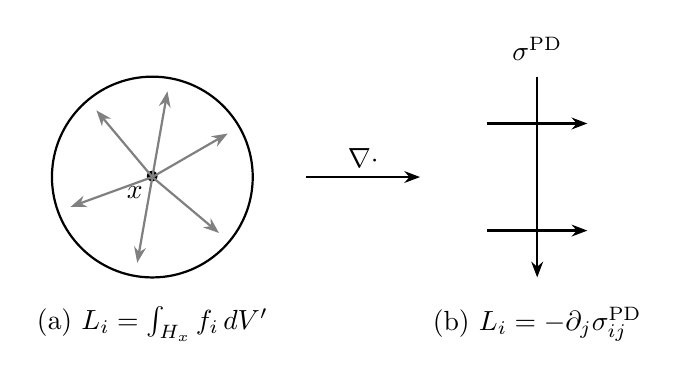
\begin{tikzpicture}[>={Stealth[length=2mm]}, scale=0.85]
% 左侧：力密度积分
\draw[thick] (0,0) circle (1.5);
\node at (0,0) {$\bullet$};
\node[below left] at (0,0) {$x$};
\foreach \a in {30,80,130,200,260,320}{
  \draw[->,gray,thick] (0,0) -- ({1.3*cos(\a)},{1.3*sin(\a)});
}
\node at (0,-2.2) {(a) $L_i=\int_{H_x}f_i\,dV'$};
% 箭头
\draw[->,thick] (2.3,0) -- (4.0,0);
\node[above] at (3.15,0) {$\nabla\cdot$};
% 右侧：应力散度
\draw[thick,->] (5,0.8) -- (6.5,0.8);
\draw[thick,->] (5,-0.8) -- (6.5,-0.8);
\draw[thick,->] (5.75,1.5) -- (5.75,-1.5);
\node[above] at (5.75,1.6) {$\sigma^{\mathrm{PD}}$};
\node at (5.75,-2.2) {(b) $L_i=-\partial_j\sigma^{\mathrm{PD}}_{ij}$};
\end{tikzpicture}
\caption{近场动力学力密度与应力散度的对应：对力在近场域 $H_x$ 上的积分（左）等价于近场动力学应力张量 $\sigma^{\mathrm{PD}}$ 散度的弱形式（右），反作用条件是建立这一等价的关键}
\label{fig:force-to-stress}
\end{figure}

\emph{AI 辅助生成，需经专业审阅。}

\section{近场动力学力密度矢量与 Cauchy 应力的关系}
\label{sec:force-cauchy}

3.2 节建立了力密度与应力散度的一般对应，但未涉及具体本构。本节针对各向同性键基模型，将近场动力学应力张量 $\sigma^{\mathrm{PD}}$ 的显式形式推导出来，并由此确定近场动力学 Lam\'e 常数与经典 Lam\'e 常数的对应关系。推导的关键一步是球面上的四阶各向同性张量积分，其系数为 $4\pi/15$，这一结果将直接导致键基泊松比 $\nu=1/4$ 的根本性约束。

\subsection{各向同性键基模型的 \texorpdfstring{$\sigma^{\mathrm{PD}}$}{sigma PD} 显式形式}
\label{subsec:isotropic-sigma}

对于各向同性键基模型，由第 2 章中心力条件 \eqref{eq:central-force}，力沿键方向，故线性化对力 $f_i=C_{ij}(\xi)\,\eta_j$ 中的微模量张量取形式
\begin{equation}
\label{eq:iso-micro-modulus}
C_{ij}(\xi) = c(r)\,\frac{\xi_i\,\xi_j}{r^2},\qquad r=|\xi|,
\end{equation}
其中 $c(r)$ 为球对称的微模量函数，描述微模量随键长的变化。此式的物理意义是：力沿键方向，大小正比于键的轴向伸长 $\eta_\parallel=\eta\cdot\xi/|\xi|$，即 $f_i=c(r)\,(\xi\cdot\eta)/r^2\cdot\xi_i$。

将近场动力学应力张量定义 \eqref{eq:pd-stress-def} 中的 $f$ 用线性化形式代入，注意 $C_{ij}=C_{ji}$（键基对称性），得
\begin{equation}
\label{eq:sigma-pd-linear}
\sigma^{\mathrm{PD}}_{ij} = \int_{|\xi|\le\delta} \xi_i\,C_{jk}(\xi)\,\eta_k\,dV_\xi = \int_{|\xi|\le\delta} c(r)\,\frac{\xi_i\,\xi_j\,\xi_k}{r^2}\,\eta_k\,dV_\xi.
\end{equation}
将一阶 Taylor 展开 $\eta_k\approx F_{kl}\,\xi_l$（$F_{kl}=\partial u_k/\partial x_l$ 为位移梯度）代入，得
\begin{equation}
\label{eq:sigma-pd-F}
\sigma^{\mathrm{PD}}_{ij} = \int_{|\xi|\le\delta} c(r)\,\frac{\xi_i\,\xi_j\,\xi_k\,\xi_l}{r^2}\,F_{kl}\,dV_\xi.
\end{equation}
换元到球坐标 $dV_\xi=r^2\,dr\,d\Omega$（$d\Omega$ 为立体角微元），记 $\hat{\xi}=\xi/r$ 为单位方向矢量，则
\begin{equation}
\label{eq:sigma-pd-sep}
\sigma^{\mathrm{PD}}_{ij} = \underbrace{\left[\int_0^\delta c(r)\,r^4\,dr\right]}_{R}\;\underbrace{\left[\int_\Omega \hat{\xi}_i\,\hat{\xi}_j\,\hat{\xi}_k\,\hat{\xi}_l\,d\Omega\right]}_{I_{ijkl}}\;F_{kl},
\end{equation}
其中 $R=\int_0^\delta c(r)\,r^4\,dr$ 是微模量的径向加权积分，$I_{ijkl}$ 是单位球面上的四阶矩。

\textbf{球面积分 $I_{ijkl}$ 的计算.}\quad 由于被积函数 $\hat{\xi}_i\hat{\xi}_j\hat{\xi}_k\hat{\xi}_l$ 在球面旋转下保持各向同性，结果必为 $\delta$ 符号的组合：
\begin{equation}
\label{eq:iso-tensor-form}
I_{ijkl} = A\bigl(\delta_{ij}\delta_{kl}+\delta_{ik}\delta_{jl}+\delta_{il}\delta_{jk}\bigr).
\end{equation}
为确定常数 $A$，对指标 $i=j$ 缩并：
\begin{equation}
\label{eq:contraction}
I_{iikl} = A\bigl(\delta_{ii}\delta_{kl}+\delta_{ik}\delta_{il}+\delta_{il}\delta_{ik}\bigr) = A\bigl(3\delta_{kl}+\delta_{kl}+\delta_{kl}\bigr) = 5A\,\delta_{kl},
\end{equation}
其中利用了 $\delta_{ii}=3$。另一方面，$\hat{\xi}_i\hat{\xi}_i=|\hat{\xi}|^2=1$，故
\begin{equation}
\label{eq:contraction-direct}
I_{iikl} = \int_\Omega \hat{\xi}_k\,\hat{\xi}_l\,d\Omega = \frac{4\pi}{3}\,\delta_{kl},
\end{equation}
后一等式是标准球面二阶矩的结果。比较得 $5A=4\pi/3$，即
\begin{equation}
\label{eq:quartic-moment}
\boxed{I_{ijkl} = \frac{4\pi}{15}\bigl(\delta_{ij}\delta_{kl}+\delta_{ik}\delta_{jl}+\delta_{il}\delta_{jk}\bigr).}
\end{equation}
此式也可通过分量直接计算验证：$I_{1111}=\int\hat{\xi}_1^4\,d\Omega=4\pi/5=3A$，$I_{1122}=\int\hat{\xi}_1^2\hat{\xi}_2^2\,d\Omega=4\pi/15=A$，均给出 $A=4\pi/15$。

\textbf{$\varepsilon$--$\omega$ 分离.}\quad 将式 \eqref{eq:quartic-moment} 代入 \eqref{eq:sigma-pd-sep} 并展开 $F_{kl}=\varepsilon_{kl}+\omega_{kl}$：
\begin{equation}
\label{eq:sigma-pd-expand}
\sigma^{\mathrm{PD}}_{ij} = \frac{4\pi R}{15}\bigl(\delta_{ij}\,\underbrace{F_{kk}}_{\varepsilon_{kk}} + F_{ij} + F_{ji}\bigr),
\end{equation}
其中 $F_{kk}=\mathrm{tr}(F)=\varepsilon_{kk}$（因 $\omega_{kk}=0$），而 $F_{ij}+F_{ji}=2\varepsilon_{ij}$（因 $\omega_{ij}+\omega_{ji}=0$）。因此 $\sigma^{\mathrm{PD}}$ 仅依赖应变 $\varepsilon$，不依赖旋转 $\omega$：
\begin{equation}
\label{eq:sigma-pd-explicit}
\boxed{\sigma^{\mathrm{PD}}_{ij} = \frac{4\pi R}{15}\,\varepsilon_{kk}\,\delta_{ij} + \frac{8\pi R}{15}\,\varepsilon_{ij},\qquad R=\int_0^\delta c(r)\,r^4\,dr.}
\end{equation}
此即各向同性键基模型的近场动力学应力张量显式形式。

\subsection{PD Lam\'e 常数与经典 Lam\'e 常数的对应}
\label{subsec:lame-correspondence}

将式 \eqref{eq:sigma-pd-explicit} 与各向同性 Hooke 定律 $\sigma_{ij}=\lambda\,\varepsilon_{kk}\,\delta_{ij}+2\mu\,\varepsilon_{ij}$ 逐项对照，得近场动力学 Lam\'e 常数
\begin{equation}
\label{eq:pd-lame}
\lambda_{\mathrm{PD}} = \frac{4\pi R}{15},\qquad \mu_{\mathrm{PD}} = \frac{4\pi R}{15},
\end{equation}
其中 $R=\int_0^\delta c(r)\,r^4\,dr$，此推导与 Silling \cite{Silling2010} 的线性化态型理论一致。表 \ref{tab:pd-ccm-correspond} 总结了近场量与经典量的对应关系。

\begin{table}[htbp]
\centering
\caption{各向同性键基近场动力学与经典弹性力学的量对应}
\label{tab:pd-ccm-correspond}
\begin{tabular}{p{0.22\textwidth}p{0.65\textwidth}}
\toprule
近场量 & 经典对应 \\
\midrule
$C_{ij}(\xi)=c(r)\,\xi_i\xi_j/r^2$ & 弹性刚度张量 $\mathcal{C}_{ijkl}=\lambda\,\delta_{ij}\delta_{kl}+\mu(\delta_{ik}\delta_{jl}+\delta_{il}\delta_{jk})$ \\
$R=\int_0^\delta c(r)\,r^4\,dr$ & Lam\'e 常数 $\lambda=\mu$ 共同的径向权重 \\
$\sigma^{\mathrm{PD}}_{ij}$ & Cauchy 应力 $\sigma_{ij}$ \\
$\lambda_{\mathrm{PD}}=\mu_{\mathrm{PD}}=4\pi R/15$ & $\lambda=\mu$（键基约束） \\
$\nu_{\mathrm{PD}}=1/4$（三维） & 泊松比 $\nu$ \\
\bottomrule
\end{tabular}
\end{table}

由 $\lambda_{\mathrm{PD}}=\mu_{\mathrm{PD}}$，泊松比为
\begin{equation}
\label{eq:nu-1-4}
\nu_{\mathrm{PD}} = \frac{\lambda}{2(\lambda+\mu)} = \frac{1}{4},
\end{equation}
此即第 2 章式 \eqref{eq:poisson-limit} 给出的键基泊松比约束。需要强调的是，此处的 $\nu=1/4$ 是三维球对称键基模型的理论上限值，并非可调参数。

\subsection{键基泊松比局限的根源}
\label{subsec:poisson-root}

$\nu=1/4$ 的根源在于键基模型仅含一个独立参数 $R$（或等价的微模量函数 $c(r)$），而经典各向同性弹性需要两个独立参数 $\lambda$ 和 $\mu$。物理上，键基模型通过键的伸缩传递力，体积变形（对应 $\varepsilon_{kk}$）与剪切变形（对应 $\varepsilon_{ij}$ 的偏斜部分）均由同一机制描述，因此 $\lambda$ 与 $\mu$ 不可独立调节。

图 \ref{fig:iso-decomp} 示意了这一约束：体积变形和剪切变形通过球对称键伸缩网络耦合到同一参数 $R$ 上，无法分别赋值。

\begin{figure}[htbp]
\centering
\begin{tikzpicture}[>={Stealth[length=2mm]}, scale=0.85]
% 左侧：体积变形
\draw[thick,dashed] (0,0) circle (1.0);
\draw[thick] (0,0) circle (1.3);
\foreach \a in {0,45,90,135,180,225,270,315}{
  \draw[->,gray,thick] (0,0) -- ({1.2*cos(\a)},{1.2*sin(\a)});
}
\node[below] at (0,-1.6) {(a) 体积变形 $\varepsilon_{kk}$};
% 中间：剪切变形
\draw[thick,dashed] (3.5,0) ellipse (1.2 and 0.8);
\draw[thick] (3.5,0) ellipse (0.8 and 1.2);
\foreach \a in {0,45,90,135,180,225,270,315}{
  \draw[->,gray,thick] (3.5,0) -- ({3.5+1.0*cos(\a)},{0.8*sin(\a)});
}
\node[below] at (3.5,-1.6) {(b) 剪切变形 $\varepsilon_{ij}$};
% 右侧：同一参数R
\draw[thick,->] (6.5,0) -- (8.0,0);
\node[above] at (7.25,0) {$R=\int c\,r^4\,dr$};
\node[below] at (7.5,-1.6) {(c) $\lambda=\mu=4\pi R/15$};
\end{tikzpicture}
\caption{键基泊松比 $\nu=1/4$ 的根源：体积变形（a）与剪切变形（b）均通过球对称键伸缩网络描述，耦合到同一径向权重 $R$（c），故 $\lambda$ 与 $\mu$ 不可独立调节}
\label{fig:iso-decomp}
\end{figure}

\begin{remark}
键基泊松比 $\nu=1/4$ 的根源在于单参数 $R$ 无法对体积模量 $K=\lambda+\tfrac{2}{3}\mu$ 和剪切模量 $\mu$ 独立赋值。Trageser 与 Seleson \cite{TrageserSeleson2020} 进一步指出，这一限制本质上是各向同性 Cauchy 关系 $C_{1122}=C_{1212}$ 在键基理论中的体现。态型理论 \cite{Silling2007} 通过引入态量（对力函数依赖键态的推广）解除了这一约束，使 $\lambda$ 与 $\mu$ 可独立调节，覆盖全范围泊松比。这一推广将在第 5 章详细讨论。
\end{remark}

\emph{AI 辅助生成，需经专业审阅。}

\section{渐近相容性}
\label{sec:asymptotic-consistency}

3.1--3.3 节建立了局部极限下的逐点对应与显式公式，但未定量刻画近场动力学解与经典弹性解之间的误差如何随 $\delta$ 趋零。本节从收敛性定理、相容性阶数、边界层效应与数值验证四个层面回答这一问题。核心结论是：在区域内部，近场动力学解与经典弹性解之差为 $O(\delta^2)$；在边界附近，存在 $O(\delta)$ 厚度的边界层，当 $\delta\to 0$ 时边界层消失。

\subsection{收敛性定理}
\label{subsec:convergence-theorem}

Silling 与 Lehoucq \cite{SillingLehoucq2008} 证明了近场动力学向经典弹性理论收敛的基本定理，Du 与 Zhou \cite{DuZhou2011} 在更弱正则性假设下给出了类似的收敛结果，其核心结论可表述如下。

\begin{theorem}[局部收敛性]
\label{thm:convergence}
设 $B$ 为 Lipschitz 区域，$u^{\mathrm{PD}}_\delta$ 为近场范围 $\delta$ 下的线性各向同性键基近场动力学方程的解，$u^{\mathrm{CCM}}$ 为相同边界条件下经典弹性方程的解。若微模量 $c(r)$ 按 $\delta$ 适当标定（使 $R=\int_0^\delta c(r)\,r^4\,dr$ 保持有限且非零），则当 $\delta\to 0$ 时
\begin{equation}
\label{eq:convergence}
\|u^{\mathrm{PD}}_\delta - u^{\mathrm{CCM}}\|_{L^2(B)} \to 0.
\end{equation}
\end{theorem}

此定理的证明思路与 3.1 节的 Taylor 展开一致：力密度 $L_i$ 的首非零项 $M_{ijkl}\,\partial_k\partial_l u_j$ 恰好等于经典应力散度 $\nabla\cdot\sigma$，高阶截断项在 $\delta\to 0$ 时趋于零。收敛的速率由截断误差的阶数决定，这正是下一小节讨论的内容。Silling 与 Lehoucq \cite{SillingLehoucq2010} 对近场动力学理论框架与收敛性有系统的综述，Dipasquale 等人 \cite{Dipasquale2014} 对这一收敛关系作了系统的理论分析与比较。

\subsection{相容性阶数}
\label{subsec:consistency-order}

由 3.1 节式 \eqref{eq:force-density-approx}，力密度的首非零项为 $M_{ijkl}\,\partial_k\partial_l u_j$，其截断误差来自 Taylor 展开中被略去的 $O(|\xi|^3)$ 项。积分后截断误差为
\begin{equation}
\label{eq:truncation-error}
\|L^{\mathrm{PD}} - \nabla\cdot\sigma\| \sim \int_{|\xi|\le\delta} C(\xi)\,|\xi|^3\,dV_\xi \sim \delta^2\,\nabla^3 u,
\end{equation}
其中 $\nabla^3 u$ 表示位移的三阶导数，最后一步利用了 $C(\xi)\sim 1/\delta^4$ 的标定（使 $R$ 有限）与积分域体积 $\sim\delta^3$。因此相容性阶数为 $O(\delta^2)$。Tupek 与 Rimoli \cite{TupekRimoli2013}、Tupek 与 Radovitzky \cite{TupekRadovitzky2014} 对近场动力学相容性阶数与收敛速率作了系统分析。

对应地，近场动力学解与经典弹性解的差异也是 $O(\delta^2)$：
\begin{equation}
\label{eq:solution-error}
\|u^{\mathrm{PD}}_\delta - u^{\mathrm{CCM}}\| \sim O(\delta^2),
\end{equation}
这一结论由 Bessa 等人 \cite{Bessa2014} 通过数值实验验证。

\subsection{边界层与表面效应}
\label{subsec:boundary-layer}

上述 $O(\delta^2)$ 的相容性阶数是在区域内部（即距边界 $\partial B$ 大于 $\delta$ 的区域）成立的。在边界附近，物质点的近场域 $H_x$ 部分落在区域 $B$ 之外，导致有效刚度 $k_{\mathrm{eff}}=\int_{H_x}C(\xi)\,dV$ 偏低，这一现象即第 2 章 2.8.2 节讨论的表面效应。

边界层的厚度为 $O(\delta)$：在距边界 $\delta$ 以内的区域，近场域被截断，力密度与应力散度的对应关系出现偏差。当 $\delta\to 0$ 且边界充分光滑时，边界层厚度趋于零，表面效应消失。图 \ref{fig:boundary-layer} 示意了这一边界层结构：区域内部近场域完整（有效刚度均匀），边界附近近场域被截断（有效刚度降低）。

\begin{figure}[htbp]
\centering
\begin{tikzpicture}[>={Stealth[length=2mm]}, scale=0.85]
% 区域B
\draw[thick] (0,0) rectangle (8,3);
\node[above right] at (8,3) {$B$};
% 边界层
\fill[gray!20] (0,0) rectangle (1.2,3);
\fill[gray!20] (6.8,0) rectangle (8,3);
\node at (0.6,1.5) {\footnotesize 边界层};
\node at (7.4,1.5) {\footnotesize 边界层};
\node at (0.6,0.3) {\footnotesize $O(\delta)$};
\node at (7.4,0.3) {\footnotesize $O(\delta)$};
% 内部
\node at (4,1.5) {\footnotesize 内部区域（$O(\delta^2)$ 相容）};
% 近场域示意
\draw[dashed] (3.5,1.5) circle (0.6);
\node[below] at (3.5,0.8) {\footnotesize $H_x$ 完整};
\draw[dashed] (0.6,1.5) circle (0.6);
\node[below] at (0.6,0.8) {\footnotesize $H_x$ 截断};
\end{tikzpicture}
\caption{近场动力学边界层结构：区域内部近场域 $H_x$ 完整，相容性阶数为 $O(\delta^2)$；边界附近 $H_x$ 被截断，有效刚度偏低，形成 $O(\delta)$ 厚度的边界层}
\label{fig:boundary-layer}
\end{figure}

第 2 章 2.8.2 节已经指出，有效刚度 $k_{\mathrm{eff}}=\int C(\xi)\,dV$ 是宏观弹性模量在近场动力学中的微观对应，其严格关系由本章 3.3 节给出。边界层内 $k_{\mathrm{eff}}$ 的偏低导致局部刚度不足，需要通过表面修正方法（如附加表面层 \cite{LeBobaru2018} 或修正微模量函数）来补偿。

\subsection{数值验证}
\label{subsec:numerical-verify}

Bessa 等人 \cite{Bessa2014} 与 Dipasquale 等人 \cite{Dipasquale2014} 对上述收敛性与相容性阶数进行了系统的数值验证。这些研究表明：在区域内部，近场动力学解与经典弹性解的相对误差随 $\delta^2$ 减小，与理论预测的 $O(\delta^2)$ 一致；在边界附近，误差增大的范围与 $O(\delta)$ 厚度的边界层吻合。图 \ref{fig:convergence-curve} 示意性地展示了这一收敛行为：在双对数坐标下，相对误差与归一化近场范围 $\delta/L$ 呈斜率为 $2$ 的线性关系，对应 $O(\delta^2)$ 收敛。

\begin{figure}[htbp]
\centering
\begin{tikzpicture}[>={Stealth[length=2mm]}, scale=1.0]
% 坐标轴
\draw[->] (0,0) -- (6.5,0) node[right] {$\delta/L$};
\draw[->] (0,0) -- (0,4.5) node[above] {相对误差};
% 网格刻度
\foreach \x in {1,2,3,4,5} \draw (\x,0) -- (\x,-0.1) node[below] {\footnotesize $10^{-\x}$};
\foreach \y in {1,2,3,4} \draw (0,\y) -- (-0.1,\y) node[left] {\footnotesize $10^{-\y}$};
% O(δ²)收敛线（斜率2）
\draw[thick,blue] (0.5,0.5) -- (5.5,3.5);
\node[blue,right] at (5.5,3.5) {\footnotesize $O(\delta^2)$};
% 标注
\node[above] at (3,2) {\footnotesize 区域内部};
\node[below right] at (6.5,0) {\footnotesize （示意）};
\end{tikzpicture}
\caption{近场动力学解与经典弹性解的相对误差随归一化近场范围 $\delta/L$ 的变化（示意性曲线）：在双对数坐标下呈斜率 $2$ 的线性关系，对应 $O(\delta^2)$ 相容性阶数，数值验证见 \cite{Bessa2014,Dipasquale2014}}
\label{fig:convergence-curve}
\end{figure}

需要强调的是，上述 $O(\delta^2)$ 的相容性阶数依赖于位移场 $u\in C^2$ 的光滑性假设。在裂纹尖端、材料界面等不连续区域，位移场可能不满足此光滑性，此时近场动力学与经典理论的差异行为将更为复杂，需要专门的分析。这正是近场动力学在处理不连续问题时的优势所在：经典理论在裂纹处遭遇奇异性困难，而近场动力学由于积分形式避免了空间导数，天然适应不连续场。

\emph{AI 辅助生成，需经专业审阅。}

\section{非局部变分原理与近场动力学方程的弱形式}
\label{sec:nonlocal-variational}

前四节从力密度、应力张量与显式本构三个层面建立了近场动力学与经典连续介质力学在逐点和渐近意义下的对应。本节换一个角度，从变分原理出发考察二者的联系。近场动力学的运动方程可以由非局部最小势能原理导出，其弱形式具有与经典 Galerkin 弱形式平行的结构，但因积分定义的非局部性，无需分部积分即可获得对称的双线性型。这一性质不仅简化了理论分析，也为近场--局部耦合方法（如 morphing \cite{Lubineau2012}）提供了天然框架。

\subsection{非局部最小势能原理}
\label{subsec:nonlocal-potential}

定义近场动力学总势能泛函
\begin{equation}
\label{eq:pd-potential}
\Pi[u] = \int_B W(u;x)\,dV - \int_B b_i\,u_i\,dV - \int_{\partial B_t}\bar{t}_i\,u_i\,dS,
\end{equation}
其中 $W$ 为第 2 章式 \eqref{eq:strain-energy} 定义的近场应变能密度（非局部积分），$b$ 为体力，$\bar{t}$ 为给定面力，$\partial B_t$ 为面力边界。与经典最小势能原理的区别仅在于 $W$ 的非局部性：$W(x)$ 依赖 $x$ 的近场域 $H_x$ 内所有物质点的位移，而非仅依赖 $x$ 处的局部应变。Javili 等人 \cite{Javili2019} 从连续介质运动学出发系统地讨论了非局部变分原理的框架。

\begin{theorem}[非局部最小势能原理]
\label{thm:nonlocal-potential}
在允许位移集 $V=\{u\in H^1(B):u|_{\partial B_u}=\bar{u}\}$ 中，平衡位移 $u$ 使 $\Pi[u]$ 取驻值，即 $\delta\Pi=0$ 当且仅当 $u$ 满足近场动力学运动方程 \eqref{eq:motion} 与面力边界条件。
\end{theorem}

\noindent\textbf{证明.}\quad 对 $\Pi$ 取变分，注意 $W$ 的变分涉及成对势 $w$ 在两端位移处的变分：
\begin{equation}
\label{eq:variation-W}
\delta W = \frac{1}{2}\int_{H_x}\bigl[\nabla_\eta w\cdot\delta u(x') + \nabla_\eta w\cdot(-\delta u(x))\bigr]\,dV',
\end{equation}
其中 $\nabla_\eta w=f$ 为对力。代入 $\delta\Pi=0$ 得
\begin{equation}
\label{eq:variation-pi}
\int_B\int_{H_x} f\cdot\bigl[\delta u(x')-\delta u(x)\bigr]\,dV'\,dV - \int_B b\cdot\delta u\,dV - \int_{\partial B_t}\bar{t}\cdot\delta u\,dS = 0.
\end{equation}
利用反作用条件 $f(x,x')=-f(x',x)$，双重积分中 $x$ 与 $x'$ 的项合并，得到 $\int_B L\cdot\delta u\,dV$，于是式 \eqref{eq:variation-pi} 等价于运动方程 $\rho\ddot{u}=L+b$ 在弱形式下的表述。$\hfill\square$

\subsection{弱形式与对称性}
\label{subsec:weak-form-symmetry}

对线性化问题，将近场动力学弱形式表述为：找 $u\in V$ 使得对所有 $v\in V_0$（$V_0$ 为齐次边界条件的允许集），
\begin{equation}
\label{eq:pd-weak-form}
a(u,v) = \ell(v),
\end{equation}
其中双线性型
\begin{equation}
\label{eq:bilinear-form}
a(u,v) = \int_B\int_{H_x} C(\xi)\,\bigl[u(x')-u(x)\bigr]\cdot\bigl[v(x')-v(x)\bigr]\,dV'\,dV,
\end{equation}
线性泛函 $\ell(v)=\int_B b\cdot v\,dV+\int_{\partial B_t}\bar{t}\cdot v\,dS$。

\textbf{对称性.}\quad 交换 $u$ 与 $v$ 的角色，$a(v,u)$ 的被积函数为 $C(\xi)[v(x')-v(x)]\cdot[u(x')-u(x)]$，与 $a(u,v)$ 的被积函数仅差内积因子的顺序，而标量内积可交换，故
\begin{equation}
\label{eq:bilinear-symmetry}
a(u,v) = a(v,u).
\end{equation}
这一对称性虽然形式上只用了内积可交换，但其物理根源在于反作用条件 $C(-\xi)=C(\xi)$ 保证了双重积分中 $x\leftrightarrow x'$ 换元下被积函数不变。对称双线性型是 Galerkin 方法稳定与收敛的理论基础。

\begin{remark}
近场动力学弱形式 \eqref{eq:pd-weak-form} 与经典弹性弱形式的关键区别在于：经典弱形式需要通过分部积分将 $\int\sigma:\varepsilon(v)\,dV$ 中的二阶导数降为一阶导数，边界项给出面力条件；而近场动力学弱形式 \eqref{eq:bilinear-form} 天然是一阶的（仅含位移差 $u(x')-u(x)$），无需分部积分。这是非局部积分形式相对于局部微分形式的结构优势。
\end{remark}

\subsection{morphing 耦合}
\label{subsec:morphing}

非局部变分原理的另一个优势是便于构造非局部--局部耦合方案。Lubineau 等人 \cite{Lubineau2012} 提出 morphing 方法，通过引入空间变化的 morphing 函数 $\alpha(x)\in[0,1]$，将总势能写为近场部分与经典部分的凸组合：
\begin{equation}
\label{eq:morphing-potential}
\Pi_{\mathrm{morph}}[u] = \int_B\bigl[\alpha(x)\,W^{\mathrm{PD}}(u;x) + (1-\alpha(x))\,W^{\mathrm{CCM}}(\varepsilon;x)\bigr]\,dV - \ell(u),
\end{equation}
其中 $\alpha=1$ 处为纯近场动力学区域，$\alpha=0$ 处为纯经典弹性区域，$\alpha$ 从 $1$ 到 $0$ 的过渡区域实现非局部--局部的光滑耦合。morphing 函数的典型设计是在边界附近设定一个 $O(\delta)$ 宽度的过渡带，使 $\alpha$ 从 $1$ 光滑衰减到 $0$。Han 等人 \cite{Han2016morphing} 将 morphing 方法推广到各向异性非局部连续体。

\begin{table}[htbp]
\centering
\caption{近场动力学与经典弹性变分原理对比}
\label{tab:variational-compare}
\begin{tabular}{p{0.22\textwidth}p{0.32\textwidth}p{0.33\textwidth}}
\toprule
特征 & 近场动力学 & 经典弹性 \\
\midrule
应变能密度 & $W=\tfrac{1}{2}\int_{H_x}w\,dV'$（非局部积分） & $W=\tfrac{1}{2}\sigma:\varepsilon$（局部） \\
弱形式 & $a(u,v)=\int\int C\,[u'-u]\cdot[v'-v]\,dV'dV$（天然一阶） & $a(u,v)=\int\sigma:\varepsilon(v)\,dV$（需分部积分降阶） \\
对称性来源 & 反作用条件 $C(-\xi)=C(\xi)$ & $\sigma$ 的对称性 $\sigma=\sigma^{\mathsf{T}}$ \\
耦合方式 & morphing 函数 $\alpha(x)$ 光滑过渡 & 分区有限元 \\
\bottomrule
\end{tabular}
\end{table}

图 \ref{fig:morphing} 示意了 morphing 耦合的结构：在区域内部使用纯近场动力学（$\alpha=1$），在边界附近通过 morphing 函数过渡到经典弹性（$\alpha=0$），兼顾近场动力学处理不连续的能力与经典弹性的计算效率。

\begin{figure}[htbp]
\centering
\begin{tikzpicture}[>={Stealth[length=2mm]}, scale=0.85]
% 区域
\draw[thick] (0,0) rectangle (10,3);
% 纯PD区域
\fill[blue!15] (1.5,0) rectangle (8.5,3);
\node at (5,1.5) {\footnotesize 纯 PD（$\alpha=1$）};
% morphing过渡
\fill[green!20] (0,0) rectangle (1.5,3);
\fill[green!20] (8.5,0) rectangle (10,3);
\node at (0.75,1.5) {\footnotesize morphing};
\node at (9.25,1.5) {\footnotesize morphing};
% α曲线
\draw[->] (0,-1.5) -- (10,-1.5) node[right] {$x$};
\draw[->] (0,-1.5) -- (0,0.5) node[above] {$\alpha(x)$};
\draw[thick,blue] (0,-1.0) -- (1.5,0.0) -- (8.5,0.0) -- (10,-1.0);
\node[below] at (0.75,-1.5) {\footnotesize $0$};
\node[below] at (5,-1.5) {\footnotesize $1$};
\node[below] at (9.25,-1.5) {\footnotesize $0$};
\node[left] at (0,0.0) {\footnotesize $1$};
\node[left] at (0,-1.0) {\footnotesize $0$};
\end{tikzpicture}
\caption{morphing 耦合示意：区域内部为纯近场动力学（$\alpha=1$），边界附近通过 morphing 函数 $\alpha(x)$ 从 $1$ 光滑过渡到 $0$，实现非局部--局部耦合 \cite{Lubineau2012}}
\label{fig:morphing}
\end{figure}

morphing 方法的优势在于过渡区域是光滑的，避免了非局部--局部界面处的反射与寄生波。其理论保证来自非局部变分原理 \eqref{eq:pd-potential} 与经典变分原理的凸组合 \eqref{eq:morphing-potential} 仍然是良定义的变分问题。Seleson 等人 \cite{SelesonParks2011} 对多种非局部--局部耦合方案进行了比较分析。

\emph{AI 辅助生成，需经专业审阅。}

本章从局部极限、近场动力学应力张量、各向同性显式本构、渐近相容性与非局部变分原理五个层面，系统建立了近场动力学与经典连续介质力学的理论联系。局部极限证明了 $\delta\to 0$ 时近场力密度退化为经典应力散度，其首非零项来自 Taylor 展开的二阶修正，由四阶张量 $M_{ijkl}$ 刻画；近场动力学应力张量 $\sigma^{\mathrm{PD}}=\tfrac{1}{2}\int(\xi\otimes f+f\otimes\xi)\,dV$ 以弱形式散度恒等式给出了力密度的局部化，其证明核心是反作用条件下的换元--相消技巧；各向同性键基模型的球面积分给出 $\sigma^{\mathrm{PD}}=(4\pi R/15)\varepsilon_{kk}\delta_{ij}+(8\pi R/15)\varepsilon_{ij}$，由此 $\lambda=\mu$，泊松比 $\nu=1/4$ 的根源在于单参数 $R$ 无法对体积与剪切变形独立赋值；渐近相容性阶数为 $O(\delta^2)$，边界层厚度为 $O(\delta)$；非局部变分原理天然无分部积分，morphing 方法实现了非局部--局部的光滑耦合。这些结果构成了第 2 章守恒律与线性化框架向具体模型的过渡桥梁，第 4 章将在此理论基础上具体化键型 PMB 模型的微弹性势、参数率定与表面效应修正。
